\chapter{Implementacja symulatora}

\par{
W poprzednich rozdziałach opisano generalne zasady wg. których powinien funkcjonować symulator środowiska miejskiego przystosowany do współpracy z systemem fuzji danych. Wskazano czym powinien się cechować by dobrze spełniać stawiane przed nim zadania - w szczególności być w stanie zapewnić dane użyteczne z punktu widzenia prowadzenia badań nad systemem fuzji danych.
}
\par{
W tym rozdziale zostanie omówiona implementacja takiego symulatora by pokazać jak w praktyce można spełnić wymagania stawiane tego rodzaju aplikacjom, jakie problemy mogą zostać napotkane i jak można sobie z nimi radzić a także jakiego rodzaju technologie można zastosować do uzyskania określonych celów.
}
\par{
W dalszej części rozdziału zostaną omówione ograniczenia tego rodzaju symulacji ze szczególnym uwzględnieniem ograniczeń wydajnościowych. Autor postara się zwrócić uwagę na największe ograniczenia takich systemów - czyli miejsca potencjalnej optymalizacji. Jednocześnie wskazane będą miejsca, które choć mogą wydawać się krytyczne z punktu widzenia symulacji przy konieczności współpracy z systemem fuzji danych przestają w ogóle odgrywać rolę, przynajmniej z punktu widzenia wydajności.
}

\section[Wymagania][Wymagania]{Wymagania}

\par{
Tak jak i inne systemy informatyczne tak i ten, choć projektowany w ramach pracy inżynierskiej musiał spełniać pewne wymagania wynikające z możliwości jego późniejszego zastosowania do badań naukowych a w szczególności do pracy Pana Macieja Grzybka dotyczącej śledzenia obiektów w systemie fuzji danych (temat pracy: "Implementacja algorytmu śledzenia obiektów w systemie fuzji danych").
}
\par{
Poniżej opisano postawione systemowi wymagania:
\begin{itemize}
	\item System powinien dostarczać informacje z czujników w mieście w formie wstępnie przetworzonej (na potrzeby fuzji informacji[?]).
	\item System powinien posiadać przynajmniej jeden typ czujnika, który dostarcza informacji w formie zawierającej co najmniej informację na temat współrzędnych geograficznych obiektu obserwowanego.
	\item System powinien udostępniać odczyty z czujników przy użyciu uzgodnionego schematu bazy danych dynamicznych (podział na bazę statyczną i dynamiczną wyjaśniony w rozdziale "Projekt bazy danych").
	\item System powinien mieć możliwość dodania implementacji bardziej zaawansowanych rodzajów czujników w szczególności posiadających inne właściwości obserwacji, dostarczające innych informacji czy też działające z określonym zaszumieniem.
	\item System powinien prezentować symulację w formie graficznej tak, by można było obserwować jej przebieg i konfrontować go organoleptycznie z wynikami dalszej analizy danych wyjściowych symulacji (ułatwienie dla wstępnej fazy prowadzenia badań).
	\item System powinien operować na danych dotyczących środowiska miejskiego pobranych z odpowiednio zdefiniowanej struktury bazy danych (wczytywanie map).
	\item System powinien umożliwiać regulację natężenia ruchu lub pozwalać na łatwe doimplementowanie tego rodzaju funkcjonalności w przyszłości.
	\item System powinien umożliwiać regulację szybkości symulacji względem czasu rzeczywistego (przyśpieszenie, spowolnienie).
	\item System powinien pozwalać na czasowe wstrzymanie symulacji.
\end{itemize}
}

\section[Metodyka symulacji][Metodyka symulacji]{Metodyka symulacji}
\subsection{Przedmiot symulacji}
\par{
Jak wspomniano w poprzednim rozdziale, dobranie skali integracji symulacji do wybranego zagadnienia jest istotne z punktu widzenia osiągnięcia zamierzonych rezultatów. Wybranie skali zbyt wysokiej ogranicza możliwości zastosowania symulacji i jej rozszerzalność. Wybranie skali zbyt niskiej skutkuje natomiast utrudnieniami implementacyjnymi, wzrostem złożoności obliczeniowej i skomplikowaniem ogólnej zasady działania symulacji bez rekompensaty w postaci użytecznych możliwości.
}
\par{
Dobranie odpowiedniej skali integracji powinno przede wszystkim uwzględniać skalę w jakiej obserwowany będzie symulowany układ, tak by w tej skali zachowywał się on realistycznie z punktu widzenia celu symulacji[?]. I tak w przypadku przedstawianego w pracy symulatora obserwowane obiekty są obserwowane w stosunkowo wysokiej skali integracji - jako samochody, piesi i inne elementy makro-świata.
}
\par{
Mając na względzie te potrzeby wydaje się więc, że można traktować te obiekty jako niepodzielne elementy i nie zagłębiać się w ich wewnętrzną specyfikę. Warto jednak uwzględnić fakt, że decyzja ta może uniemożliwiać lub w znacznym stopniu utrudniać niektóre przyszłe rozszerzenia symulacji. I tak jak nie będzie zapewne stanowiło problemu dodanie do symulacji obsługi zderzeń niesprężystych gdyż ich obsługa nie wymaga zagłębiania się w budowę obiektów, tak obsługa np. aerodynamiki pojazdów może stanowić znaczące utrudnienie implementacyjne. Należy pamiętać, że nie każde obliczenia mikro skali da się przełożyć na wartości w skali makro [?].
}
\par{
Licząc się z wyżej wspomnianymi konsekwencjami podjęto decyzję, by elementy świata rozpatrywać w skali abstrakcyjnych obiektów o nieznanej wewnętrznej budowie. Będąc świadomym, iż przedmiotem naszej symulacji są właśnie obiekty makro-świata zawieszone w czterowymiarowej przestrzeni (przestrzeń i czas) i będąc świadomym ich właściwości można przystąpić do dalszego planowania metodyki symulacji.
}

\subsection{Model symulacji}
\par{
Poprzedni podrozdział uzasadnił dlaczego przy implementacji symulatora zdecydowano się na nie wgłębianie w wewnętrzną strukturę obiektów a jedynie zasymulowanie ich poprawnego z punktu widzenia celu symulacji zachowania w możliwie prosty sposób. Innym problemem z jakim należało sobie poradzić było ustalenia jak przedstawić owe makroskopowe obiekty by zachowywały się one w sposób realistyczny z punktu widzenia informacji istotnych dla obserwatorów.
}
\par{
Z pomocą przy rozwiązaniu tego problemu przychodzi nam teoria symulacji a także podstawy dynamiki Newtona przedstawione w pierwszym rozdziale.
I tak wiemy, że zastosowanie właśnie modelu newtonowskiego do symulowania ruchów obiektów da nam obraz realistyczny z punktu widzenia makro świata.
}
\par{
Podstawowymi wielkościami dynamiki Newtona są siła (F), przyśpieszenie (a) oraz masa (m), połączone wzorem:
\begin{center}
$F = m \times a$
\end{center}
Wzór ten opisuje podstawę ruchu i odnosi się właśnie do obiektów makroskopowych o nieznanej lub nieokreślonej strukturze wewnętrznej opisywanych modelami fizycznymi takimi jak punkt materialny lub bryła sztywna.
}
\par{
Dla ciał opisywanych przy użyciu symulatora również należało znaleźć odpowiedni model fizyczny. Pod uwagę wzięto dwa wyżej wspomniane modele, jako, że zapewniają one realizm symulacji i pozwalają na uwzględnianie licznych czynników zewnętrznych.
}
\par{
Podejście do obiektów symulowanych jak do bryły sztywnej wydaje się być intuicyjne. W naturalny sposób blokuje to możliwość ingerencji w wewnętrzną fizykę ciała, jednocześnie zapewniając wysoki realizm w skali makro.
Takie podejście pozwala na łatwe zasymulowanie wszelkiego rodzaju zdarzeń niesprężystych, także związanych z obrotami, w sposób naturalny ułatwia wykrywanie kolizji i pozwala przewidywać ich przebieg z dużą dokładnością i z zachowaniem wysokiego realizmu.
Niestety model ten ze względu na stopień kompilacji został odrzucony a wybrany został model prostszy - model punktu materialnego.
\par{
Model punktu materialnego pozwala na wykonywanie wszelkich obliczeń na obiektach które nie nawiązują między sobą interakcji równie dobrze jak model bryły sztywnej. Jego niewątpliwą wadą jest to, że w razie pojawienia się potrzeby symulowania zderzeń między obiektami pojawił by się spory narzut na dość sztucznej warstwie abstrakcji, która musiała by powstać by obsłużyć zderzenia w sposób realistyczny (dodać do modelu odpowiednie siły itp.).
Ponadto model ten nie uwzględnia w ogóle obrotów, ponieważ z jego punktu widzenia obiekty w świecie stają się niematerialnymi punktami bez wymiarów.
Największą i przeważającą zaletą tego modelu była jego prostota, która pozwoliła na szybką implemetację wersji symulatora zdolnej spełniać podstawowe powierzone jej zadania. 
}
\par{
W ramach modelu fizyki punktu materialnego przyjęto, że każdy obiekt w świecie stanowi jeden punkt materialny, który w każdej chwili czasu charakteryzuje się następującymi wartościami:
\begin{itemize}
\item Siła (wektor trójwymiarowy) z jaką działa ciało na świat stanowiący inercjalny układ odniesienia rozumiany jako statyczny obiekt o nieskończonych wymiarach, względem, którego przemieszczają się ciała (swoista podstawa układu).
\item Masa ciała
\item Prędkością (wektor trójwymiarowy) z jaką w danej chwili porusza się ciało.
\end{itemize}
Znając te trzy wartości w każdej chwili czasu na podstawie modelu fizycznego można określić położenie obiektu w układzie współrzędnych w każdej chwili czasu.
Warto zwrócić uwagę, że tak jak pierwsze dwa z tych parametrów są właściwościami obiektu tzn. obiekt może je dowolnie zmieniać w czasie, tak prędkość jest wartością wynikającą z dotychczasowej historii danego obiektu i sam obiekt nie jest w stanie wprost zmienić jej wartości (tak jak w rzeczywistości samochód nie może w jednej chwili się zatrzymać, ale może nagle (w modelu przyjęto że nawet w czasie $\Delta t \longrightarrow 0$) zacząć hamować działając z dużą siłą o zwrocie przeciwnym do kierunku jazdy i szybko (ale nie natychmiastowo) wytracić posiadaną prędkość).
}

\subsection{Upływ czasu}
\par{
Ostatnią z punktu widzenia istoty symulacji decyzją jaką należało podjąć było wybranie jednego z dwóch możliwych podejść do symulowania upływu czasu:

\begin{itemize}
\item Obliczenia przy założeniu ciągłości czasu
\item Obliczenia przy założeniu czasu skwantowanego (dyskretnego)
\end{itemize}
}
\par{
Pierwsze z podejść jest bliższe realizmowi (choć w świetle współczesnych badań fizycznych okazuje się, że czas należy rzeczywiście traktować jako parametr zdyskretyzowany, to gęstość jego rzeczywistego "próbkowania" jest tak duża, że nie sposób obsługiwać ją przy użyciu komputera).
Jak wspominano w poprzednim rozdziale, uzyskanie efektu czasu ciągłego sprowadza się do opisania wszystkich elementów symulowanego świata układem równań. W każdej chwili pozycja każdego obiektu może być wyznaczona jako pozycja początkowa przesunięta o wektor wyznaczany z bieżącego równania ruchu danego ciała. Tego rodzaju symulacja zapobiega wszelkiego rodzaju błędom przybliżeń i błędom kwantowania, ma ona jednak inne właściwości, które dyskwalifikują jej użycie.
}
\par{
Warto zwrócić uwagę, że tego typu równania wyznacza się ponownie ilekroć pojawia się jakiegoś rodzaju zdarzenie. Przez zdarzenie rozumie się tutaj wszelkie sytuacje mogące wpływać na stan jakiegokolwiek ciała. I tak podstawowymi zdarzeniami w typowym modelu fizycznym są np. zderzenia dwóch ciał. W wypadku symulacji zdarzenie następuje jednak również wtedy gdy co najmniej jeden z obiektów zechce pod wpływem czynników zewnętrznych zmienić swój stan (tj. siłę lub masę). Niestety wyznaczanie tego rodzaju momentów w czasie wydaje się być zadaniem bardzo trudnym. Po pierwsze nie jesteśmy w stanie przewidzieć w jakich sytuacjach obiekt będzie chciał zmieniać swój stan - musimy więc przenieść tę odpowiedzialność na niego. Po drugie obiekt taki musi w swoisty sposób przewidywać przyszłość by zaplanować zdarzenie - każdy obiekt musi więc mieć pojęcie o całym układzie by być w stanie (i to przy dużym nakładzie obliczeniowym) przewidzieć i zaplanować zdarzenia, które dotyczą jego stanu ruchu.
}
\par{
Rozwiązaniem, które pozwoliło by wdrożyć ideę czasu ciągłego w życie bez konieczności wprowadzania olbrzymiej ilości obliczeń, jest twarde zdefiniowanie w modelu sytuacji w których poszczególne obiekty mogą zmieniać decyzje. Warto jednak zwrócić uwagę, że zmniejsza to decyzyjność pojedynczych jednostek w świecie co obniża realizm ewentualnie wdrożonej sztucznej inteligencji.
}
\par{
Wyżej wspomniane powody sprawiły, iż zdecydowano się na wybranie wariantu symulacji z czasem jako jednostką skwantowaną. W takiej sytuacji każdy kwant jest punktem decyzji dla każdego obiektu a przez okres jego trwania ciała poruszają się ze stałymi parametrami (przyśpieszenie, prędkość).
Takie rozwiązanie posiada szereg wad. Po pierwsze, w przypadku potrzeby zasymulowania kolizji pojawia się problem nachodzenia na siebie obiektów. W typowym przypadku zderzenia, w jednym kwancie czasu dwa ciała będą rozłączne a w następnym momencie będą się na siebie nakładały. Jest to niezgodne z modelem fizycznym bryły sztywnej jak i intuicją jednak istnieją sposoby radzenia sobie z tego rodzaju problemami - nie są one jednak przedmiotem tej pracy a ponieważ w załączonej implementacji zrezygnowano z obsługi zderzeń, nie będą one tutaj rozpatrywane - warto jednak mieć na względzie ograniczenie samej metodyki symulowania upływu czasu.
}
\par{
Kolejny problem pojawiający się przy obsłudze czasu w kwantach przy zachowaniu szybkości jego upływu w stosunku do czasu rzeczywistego jest fakt, że przy dużym czasie zajmowanym przez każdy krok (np. na skutek operacji IO) algorytmu odpowiadający kwantowi czasu, wydłuża się czas jego trwania w symulacji. W skrajnych wypadkach może to doprowadzić do kwantów czasu bardzo długich co sprawia, że błąd kwantowania staje się ogromny - w praktyce może to np. powodować opuszczenie przez obiekty obszaru symulacji.
Problem ten można oczywiście zlikwidować rezygnując z odniesienia czasu symulacji do czasu rzeczywistego (wtedy błąd kwantowania jest stały i z założenia niewielki), jednak jako że takie odniesienie jest jednym z wymagań stawianym symulatorowi, tego typu sytuacje mimo ich nieprecyzyjności należało w jakiś (możliwe realistyczny z punktu widzenia obserwacji) sposób obsłużyć, a na pewno nie należało ich podczas dalszej implementacji zaniedbać. Zaproponowane rozwiązanie i konkretne miejsca występowania tego problemu opisano w dalszej części pracy.
}
\par{
Dobranie metodyki obsługi upływu czasu stanowi zwieńczenie procesu projektowania działania symulatora. W jego wyniku otrzymano obraz symulatora jako procesu działającego na abstrakcyjnych obiektach makro-świata, obsługiwanych zgodnie z zasadami dynamiki newtona tak jakby były punktami materialnymi przy jednoczesnym zachowaniu kwantyzacji czasu pozwalającej na swobodne zmiany stanu (rozumianego jako masa i siła) obiektów na skutek ich własnych decyzji w wyznaczonych momentach czasu symulacji.
}

\section[Dobór technologii][Dobór technologii]{Dobór technologii}
\par{
Elementem implementacji aplikacji jest dobranie technologii odpowiadającej wymaganiom stawionym aplikacji. Przez technologie rozumie się w tym wypadku przede wszystkim język programowania oraz system baz danych służący do komunikacji z systemem fuzji danych jak i ten mający odpowiadać za statyczne informacje dotyczące symulowanego środowiska (układ ulic, budynków itp).
Poniższy rozdział traktuje o doborze tych technologii opisując powody ich wyboru.
}
\subsection{Wybór języka programowania}
\subsubsection{Rozszerzalność}
\par{
Symulator według wyżej wyspecyfikowanych wymagań ma na wielu płaszczyznach wspierać możliwości rozszerzania. Obecnie za paradygmat programowania umożliwiający rozszerzenie funkcjonalności w największym stopniu uważa się paradygmat programowania obiektowego.
W związku z tym pod uwagę w wyborze brane będą tylko języki programowania związane z tym paradygmatem a jednocześnie znane choć w podstawowym stopniu autorowi niniejszej pracy:
\begin{itemize}
\item C++
\item Java
\item C\#
\end{itemize}
}
\subsubsection{Dostępność}
\par{
Istotnym elementem z punktu widzenia każdej aplikacji użytkowej, także tej tworzonej z myślą o prowadzeniu badań naukowych zdaje się być możliwość wykorzystania jej na różnych platformach sprzętowo-systemowych.
}
\par{
I tak spośród wymienionych wcześniej języków programowania tylko dwa pierwsze zdają się pokrywać zakresem swej dostępności porównywalne ilości platform - są to Java, której kod ze względu na wykorzystanie implementowanej na wiele popularnych platform wirtualnej maszyny może być wykonywany na większości współczesnych urządzeń elektronicznych (nie tylko klasy PC), oraz C++, którego kompilacja i wykonanie ze względu na szeroko dostępne kompilatory dla wielu architektur oraz implementacje biblioteki standardowej nie stanowi problemu dla większości popularnych konfiguracji sprzętowo-systemowych.
}
\par{
Niestety język C\# zdaje się nie być równie dostępny na wielu platformach. Implementacje jego wirtualnej maszyny nie są zbyt szeroko dostępne a nawet jeśli istnieją są generalnie postrzegane jako półśrodek nie do końca spełniający swoją rolę. Z tego względu język C\# został odrzucony i nie będzie rozpatrywany w kolejnych kategoriach doboru.
}
\subsubsection{Wydajność}
\par{
Choć wydajność obliczeń nie jest kluczowym elementem dla aplikacji, czego dowiodły późniejsze badania, to czas obliczeń jest niewątpliwym kosztem w związku z tym jego minimalizacja zdaje się być istotnym elementem decyzyjnym przy doborze języka programowania.
}
\par{
Język C++ jako język kompilowany bezpośrednio (lub pośrednio) do kodu natywnego kodu maszynowego daje możliwość uzyskania idealnie optymalnego kodu dla danego rozwiązania na danej platformie sprzętowej. W tej kategorii język Java, będący językiem kompilowanym do maszyny wirtualnej z natury rzeczy uzyska niższe wyniki wydajnościowe - ze względu niemożliwą do uniknięcia dodatkową warstwę interpretacji w trakcie wykonywania.
}
\par{
Przewaga języka C++ nad Javą jest niezaprzeczalna, jednakże wydajność nie jest głównym kryterium doboru technologii w związku z tym nie wydaje się by odrzucenie języka Java na tym etapie było rozsądną koncepcją.
}
\subsubsection{Doświadczenie}
\par{
Istotne z punktu widzenia tworzenia aplikacji jest doświadczenie programistyczne w danej technologii. Ogranicza ono błędy. Skraca czas potrzebny na implementację. Pozwala uniknąć nawrotów. Doświadczony w danej technologii ma większą szansę na stworzenie bezawaryjnego i utrzymywalnego oprogramowania.
}
\par{
Doświadczenie autora jest zdecydowanie po stronie języka C++, który jest dla niego naturalnym narzędziem pracy. Język Java znany jest mu tylko pobieżnie i w związku z tym zdaje się on być w tym kontekście mniej rozsądnym wyborem.
}
\subsubsection{Odporność na błędy}
\par{
Naturalną rzeczą związaną nieodłącznie z wytwarzaniem jakiegokolwiek oprogramowania są błędy programistyczne. Języki różnego typu w różny sposób bronią się przed nimi swoją strukturą.
}
\par{
Zarówno język Java jak i język C++ są językami silnie typowanymi. Oznacza to, że za błąd w ich kontekście uważa się zachowania powszechnie uznawane za nielogiczne - stawianie obiektów złych klas w określonych kontekstach. Języki te bronią nas więc przed błędami, których znakomitym podsumowaniem jest żart \textit{"Jechały dwa autobusy jeden był zielony a drugi też skręcał w prawo."}.
}
\par{
Aspektem typowym dla języka C++, który został wyeliminowany w języku Java jest ręczne zarządzanie pamięcią, które uznawane jest powszechnie za najbardziej błędogenny element tworzenia oprogramowania. W związku z tym, należy zwrócić uwagę, że w tej kwestii język Java, który sam obsługuje pamięć nie obciążając tym programisty wydaje się być zauważalnie lepszy.
}
\subsubsection{Wybór}
\par{
Mając na względzie powyższe elementy oceny, wybór wydaje się być nietrywialny. Wydajność w dzisiejszych czasem nie jest specjalnym kosztem a dla tego konkretnego projektu nie jest kluczowa zwłaszcza jeśli mówimy tylko o zmianach w obrębie tego samego rzędu wielkości. Jednocześnie język chroniący programistę przed jego własnymi błędami zdaje się mieć tu zauważalną przewagę. W praktyce jednak najbardziej kluczowe zdaje się być doświadczenie programistyczne autora tej pracy, które zaważyło o wyborze języka C++.
}

\subsection{Wybór silnika bazy danych}
\par{
Pod uwagę brano następujące silniki baz danych:
\begin{itemize}
\item ORACLE DB
\item PostgreSQL
\item MySQL
\item sqLite
\end{itemize}
}

\subsection{Wybór technologii tworzenia interfejsu}
\par{
Wybór technologii interfejsu nie był kluczowy dla projektu, dlatego autor wybrał w zasadzie jedyną dobrze znaną sobie bibliotekę umożliwiającą tworzenie przenośnych interfejsów graficznych --- bibliotekę Qt. Biblioteka zdawała się być wystarczająco dobrym rozwiązaniem w związku z czym poszukiwanie alternatywnych rozwiązań wydawało się bezzasadne zwłaszcza, że prezentowanie wyników symulacji nie jest kluczowe z punktu widzenia celu pracy.
}

\section[Projekt bazy danych][Projekt bazy danych]{Projekt bazy danych}
\par{
W ramach symulatora wykorzystywane są dwie odrębne bazy danych. Jedna (baza danych dynamicznych) stanowi główne wyjście aplikacji i służy do zapisu odczytów z czujników umieszczonych wewnątrz symulacji. Druga z baz - baza statyczna - służy do opisywania środowiska miejskiego a w zasadzie jego statycznych elementów.
}

\subsection{Baza danych statycznych}
\par{
Zadaniem bazy danych statycznych jest przechowywanie układu ulic, budynków w symulowanym środowisku miejskim. Symulator w pierwszej fazie swojego działania (inicjalizacji) będzie wczytywał tego rodzaju dane by pracować na nich przez cały czas symulacji.
}
\par{
Kwestią dyskusyjną było umieszczenie w bazie danych statycznych umiejscowienia czujników, ponieważ mają one charakter odpowiadający jej specyfice (są niezmienne przez cały czas symulacji). Jednakże, ze względu na to, że do danych tych odnosi się baza dynamiczna, by uniknąć niepotrzebnej zależności jednej bazy od drugiej zdecydowano by umiejscowienie czujników przenieść do bazy danych dynamicznych.
}
\par{
Baza danych statycznych zawiera więc:
\begin{itemize}
\item Układ ulic - rozumiany jako graf geometryczny
\item Umiejscowienie i kształt budynków - traktowanych jako graniastosłupy
\end{itemize}
Szczegóły bazy można zobaczyć na diagramie ER poniżej.
}

\par{
\begin{center}
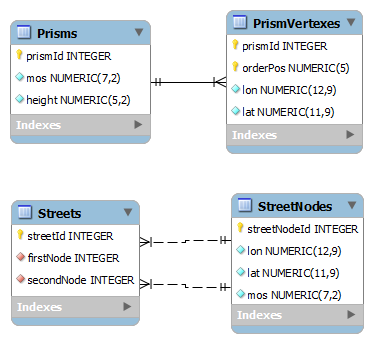
\includegraphics[width=25em]{img/static_db}
\end{center}
}
\par{
\begin{center}
\textit{Diagram ER bazy danych statycznych.}
\end{center}
}

\subsection{Baza danych dynamicznych}
\par{
}

\section[Architektura systemu][Architektura systemu]{Architektura systemu}
\par{ Treść... }
\subsection{Model MVC}
\subsubsection{O modelu}
\subsubsection{Zastosowanie w aplikacji}
\subsection{Wielowątkowość}
\subsubsection{Biblioteka boost::thread}
\subsubsection{Problemy synchronizacji}

\section[Architektura modelu][Architektura modelu]{Architektura modelu}
\par{ Treść... }
\subsection{Obiekty świata}
\subsection{Interakcja między obiektami}
\subsubsection{Wzorzec wizytatora}
\subsection{Upływ czasu}
\subsubsection{Biblioteka boost::chrono}
\subsubsection{Wzorzec obserwatora}
\subsection{Połączenie z bazą danych}
\subsubsection{Biblioteka pqxx}
\subsubsection{ORM}
\subsection{Komunikacja ze światem (API)}
\subsubsection{Metody publiczne}
\subsubsection{Wołania asynchroniczne}
\subsubsection{Obserwacja stanu symulacji}

\section[Architektura widoku][Architektura widoku]{Architektura widoku}
\par{ Treść... }
\subsection{Biblioteka Qt}
\subsubsection{Wymagania biblioteki}
\subsubsection{QGraphicsLibrary}
\subsubsection{Architektura sygnał-slot}
\subsection{Projektowanie interfejsu graficznego}
\subsubsection{Tworzenie własnych widżetów}

\section[Architektura kontrolera][Architektura kontrolera]{Architektura kontrolera}
\par{ Treść... }
\subsection{Odcięcie od biblioteki Qt}
\subsection{Klasy zdarzeń i ich obsługa}
\subsection{Kolejki a architektura sygnał-slot}